
% LaTeX Language and campus name and format package
\documentclass[es,gi]{ifirak}\usepackage[]{graphicx}\usepackage[]{color}
%% maxwidth is the original width if it is less than linewidth
%% otherwise use linewidth (to make sure the graphics do not exceed the margin)
\makeatletter
\def\maxwidth{ %
  \ifdim\Gin@nat@width>\linewidth
    \linewidth
  \else
    \Gin@nat@width
  \fi
}
\makeatother

\definecolor{fgcolor}{rgb}{0.345, 0.345, 0.345}
\newcommand{\hlnum}[1]{\textcolor[rgb]{0.686,0.059,0.569}{#1}}%
\newcommand{\hlstr}[1]{\textcolor[rgb]{0.192,0.494,0.8}{#1}}%
\newcommand{\hlcom}[1]{\textcolor[rgb]{0.678,0.584,0.686}{\textit{#1}}}%
\newcommand{\hlopt}[1]{\textcolor[rgb]{0,0,0}{#1}}%
\newcommand{\hlstd}[1]{\textcolor[rgb]{0.345,0.345,0.345}{#1}}%
\newcommand{\hlkwa}[1]{\textcolor[rgb]{0.161,0.373,0.58}{\textbf{#1}}}%
\newcommand{\hlkwb}[1]{\textcolor[rgb]{0.69,0.353,0.396}{#1}}%
\newcommand{\hlkwc}[1]{\textcolor[rgb]{0.333,0.667,0.333}{#1}}%
\newcommand{\hlkwd}[1]{\textcolor[rgb]{0.737,0.353,0.396}{\textbf{#1}}}%
\let\hlipl\hlkwb

\usepackage{framed}
\makeatletter
\newenvironment{kframe}{%
 \def\at@end@of@kframe{}%
 \ifinner\ifhmode%
  \def\at@end@of@kframe{\end{minipage}}%
  \begin{minipage}{\columnwidth}%
 \fi\fi%
 \def\FrameCommand##1{\hskip\@totalleftmargin \hskip-\fboxsep
 \colorbox{shadecolor}{##1}\hskip-\fboxsep
     % There is no \\@totalrightmargin, so:
     \hskip-\linewidth \hskip-\@totalleftmargin \hskip\columnwidth}%
 \MakeFramed {\advance\hsize-\width
   \@totalleftmargin\z@ \linewidth\hsize
   \@setminipage}}%
 {\par\unskip\endMakeFramed%
 \at@end@of@kframe}
\makeatother

\definecolor{shadecolor}{rgb}{.97, .97, .97}
\definecolor{messagecolor}{rgb}{0, 0, 0}
\definecolor{warningcolor}{rgb}{1, 0, 1}
\definecolor{errorcolor}{rgb}{1, 0, 0}
\newenvironment{knitrout}{}{} % an empty environment to be redefined in TeX

\usepackage{alltt}

% ERABILIKO DIREN PAKETEAK %

% listings pakage is for code formating
\usepackage{listings}
% Paquete for acents and other special characters
% It is not necesary to use all this packages add or remove those you are interested on
\usepackage[utf8]{inputenc}
\usepackage[table]{xcolor}
\usepackage{graphicx}
\usepackage{wrapfig}
\usepackage{amsfonts}
\usepackage{makeidx}
\usepackage{adjustbox}
\usepackage{booktabs}
\usepackage{amsmath}
% Custom colors
\usepackage{color}
\usepackage{pythonhighlight}
%
%%PYthon
%\definecolor{deepblue}{rgb}{0,0,0.5}
%\definecolor{deepred}{rgb}{0.6,0,0}
%\definecolor{deepgreen}{rgb}{0,0.5,0}
%
%% Default fixed font does not support bold face
%\DeclareFixedFont{\ttb}{T1}{txtt}{bx}{n}{12} % for bold
%\DeclareFixedFont{\ttm}{T1}{txtt}{m}{n}{12}  % for normal
%
%% Python style for highlighting
%\newcommand\pythonstyle{\lstset{
%language=Python,
%basicstyle=\ttm,
%otherkeywords={self},             % Add keywords here
%keywordstyle=\ttb\color{deepblue},
%emph={MyClass,__init__},          % Custom highlighting
%emphstyle=\ttb\color{deepred},    % Custom highlighting style
%stringstyle=\color{deepgreen},
%frame=tb,                         % Any extra options here
%showstringspaces=false            % 
%}}
%
%
%% Python environment
%\lstnewenvironment{python}[1][]
%{
%\pythonstyle
%\lstset{#1}
%}
%{}
%
%% Python for external files
%\newcommand\pythonexternal[2][]{{
%\pythonstyle
%\lstinputlisting[#1]{#2}}}
%
%% Python for inline
%\newcommand\pythoninline[1]{{\pythonstyle\lstinline!#1!}}

% USAGE OF PYTHON
%
%\section{``In-text'' listing highlighting}
%
%\begin{python}
%class MyClass(Yourclass):
%    def __init__(self, my, yours):
%        bla = '5 1 2 3 4'
%        print bla
%\end{python}
%
%\section{External listing highlighting}
%
%\pythonexternal{demo.py}
%
%\section{Inline highlighting}
%
%Definition \pythoninline{class MyClass} means \dots


\DeclareMathSizes{10}{10}{10}{10}

\graphicspath{imagenes}
\renewcommand{\contentsname}{Indice}
\IfFileExists{upquote.sty}{\usepackage{upquote}}{}
\begin{document}

% Course year
\ikasturtea{2018 - 2019}
% Subject or course name
\irakasgaia{Visión por Computador}
% Title
\title{Desafío 11}
% Name of Author
\author{Mikel Dalmau}

\maketitle



%\section{Código}

\tableofcontents

\section{Enunciado}
\paragraph{}El objetivo de este desafío es realizar una aplicación que detecte la pupila del ojo en  vídeo de tiempo real utilizando la API de OpenCV.\\

El proceso propuesto, asumiendo que la imagen de  contiene uno de los ojos completamente, aplicar el detector de ojos basado en clasificadores en cascada proporcionado por OpenCV (tutorial-99). Este detector proporciona una región de la imagen conteniendo el ojo. Aplicar la transformada de Hough circular para encontrar la pupila. posiblemente tras procesos de extracción de bordes (tutorial-19) y eliminación de ruido usando procesos morfológicos (tutorial-17).\\

Resultado del trabajo debería ser un vídeo anotado con las detecciones y la secuencia temporal de los radios de los círculos detectados.\\

\pagebreak
\section{Clasificador en cascada}
\paragraph{}En la aplicación utilizo dos detectores basados en clasificadores en cascada exactamente igual que en el tutorial-99 proporcionado por Opencv.\\
 
\begin{figure}[hbtp]
\centering
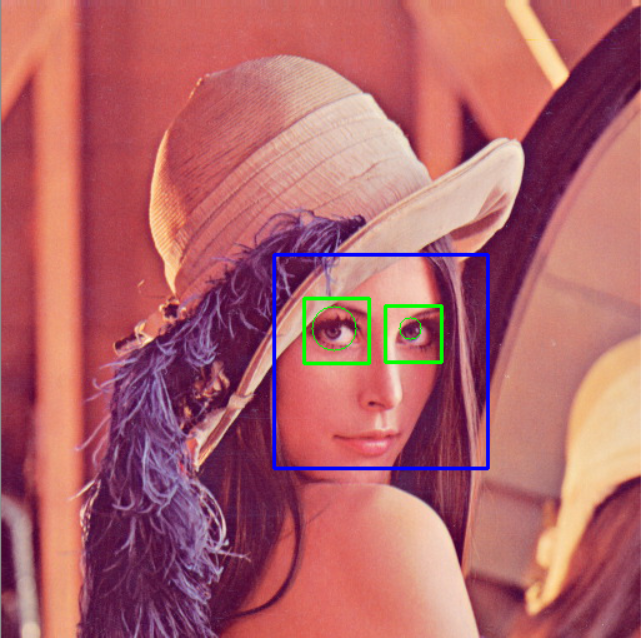
\includegraphics[scale=0.5]{imagenes/cascada.png}
\caption{Resultado aplicación de detectores tutorial-99}
\end{figure}

Con esto, logro las regiones de interés de ambos ojos y así puedo aplicar la transformada de Hough sobre un espacio mucho más localizado, mejorando la eficiencia y resultados.\\

\begin{python}
# Para cada cara hallada, extraer la region de interes
    faces = face_cascade.detectMultiScale(gray, 1.3, 5)
    for (x,y,w,h) in faces:
        roi_gray = gray[y:y+h, x:x+w]
        roi_color = frame[y:y+h, x:x+w]
       
        # Para cada ojo, extraer la region de interes
        eyes = eye_cascade.detectMultiScale(roi_gray)
        for (ex,ey,ew,eh) in eyes:
            roi_eyes = roi_color[ey:ey+eh, ex:ex+ew]
            roi_eyes_gray = roi_gray[ey:ey+eh, ex:ex+ew]
\end{python}

\section{Transformaciones Morfológicas}
\paragraph{}
En las siguientes páginas se muestras los resultados de aplicar distintas transformaciones morfológicas a los bordes de dos tipos distintos de ojos.\\
 
Aunque no he tenido tanto en cuenta estos resultados, me he decidido por utilizar la transformación Opening o Apertura que es una combinación de una erosión seguida de una dilatación y es útil para eliminar el ruido de las imágenes ampliando también el blanco del ojo en la dilatación y por lo tanto aislando la pupila.\\

\pagebreak
\begin{center}
\begin{tabular}{p{2cm} p{2cm} c c}
    \toprule 
    	\bfseries Morfología
    	& \bfseries Kernel
    	& \bfseries Resultado
    	& \bfseries Transformada de Hough\\

    	closing
    	& 4x4
		& \adjustimage{height=4cm,valign=m}{imagenes/closing_i_x}
		& \adjustimage{height=4cm,valign=m}{imagenes/closing_i_o}\\
		
		gradient
		& 4x4
		& \adjustimage{height=4cm,valign=m}{imagenes/gradient_d_x}
		& \adjustimage{height=4cm,valign=m}{imagenes/gradient_d_o}\\
	
		open
		& 3x3
		& \adjustimage{height=4cm,valign=m}{imagenes/open_d_x}
		& \adjustimage{height=4cm,valign=m}{imagenes/open_d_o}\\

		open
		& 3x3
		& \adjustimage{height=4cm,valign=m}{imagenes/open_i_x}
		& \adjustimage{height=4cm,valign=m}{imagenes/open_i_o}\\
	
		close
		& 3x3
		& \adjustimage{height=4cm,valign=m}{imagenes/close_d_x}
		& \adjustimage{height=4cm,valign=m}{imagenes/close_d_o}\\
		
    \bottomrule
\end{tabular}
\end{center}

\begin{center}
\begin{tabular}{p{2cm} p{2cm} c c}
    \toprule 
    	\bfseries Morfología
    	& \bfseries Kernel
    	& \bfseries Resultado
    	& \bfseries Transformada de Hough\\
	
		close
		& 3x3
		& \adjustimage{height=4cm,valign=m}{imagenes/close_i_x}
		& \adjustimage{height=4cm,valign=m}{imagenes/close_i_o}		
		\\
		
		dilate
		& 3x3
		& \adjustimage{height=4cm,valign=m}{imagenes/dilate_i_x}
		& \adjustimage{height=4cm,valign=m}{imagenes/dilate_i_o}	\\
	
		dilate
		& 3x3
		& \adjustimage{height=4cm,valign=m}{imagenes/dilate_d_x}
		& \adjustimage{height=4cm,valign=m}{imagenes/dilate_d_o}\\
		
		erode
		& 3x3
		& \adjustimage{height=4cm,valign=m}{imagenes/erode_i_x}
		& \adjustimage{height=4cm,valign=m}{imagenes/erode_i_o}			
		\\
		
		erode
		& 3x3
		& \adjustimage{height=4cm,valign=m}{imagenes/erode_d_x}
		& \adjustimage{height=4cm,valign=m}{imagenes/erode_d_o}			
		\\
								
    \bottomrule
\end{tabular}
\end{center}

\section{Transformada de Hough Circular}
\paragraph{}Finalmente, para detectar la pupila utilizo la transformada de Hough circular y para ello me valgo de la siguiente función.\\

Cabe destacar de esta función los parámetros param1 y param2, ya que internamente HoughCircles llama a la función Canny del tutorial 19 para la extración de bordes y es con estos parametros que controlamos esta función. Sin entrar más en ello e determinado por prueba y error unos parámetros que resultaban aceptables.\\

\begin{python}
                # aplicar una transformacion morfologica y la transformada de Hough Circular
                roi_eyes_gray  = cv2.morphologyEx(roi_eyes_gray, cv2.MORPH_OPEN, kernel)
                circles = cv2.HoughCircles(roi_eyes_gray,cv2.HOUGH_GRADIENT,1,30,param1=100,param2=20,minRadius=5,maxRadius=50)
\end{python}

\section{Resultados}
\paragraph{} Finalmente tras solucionar los problemas relacionados con los códecs de vídeos y otros detalles he creado un par de vídeos con la detección de pupilas en tiempo real, se llaman desafío11-erode y desafío11-open y en cada uno se ha utilizado una de las transformaciones morfológicas.\\

En la siguiente tabla se muestran los radios obtenidos en cada momento del vídeo, en caso de detectarse un ojo pero no la pupila, el radio es asignado el valor -1, en caso de no detectarse nada no no se asigna valor como puede apreciarse por el bloque blanco en una de las imágenes, ya que giro la cabeza en medio del vídeo.\\

Por otro lado, en el primer gráfico, se trata de un vídeo en el que miro en distintas direcciones lo que explica las variaciones en el gráfico pero la media de los radios es similar en ambos y mayor que que el tamaño original de la pupila.\\


\begin{center}
\begin{tabular}{c c}
    	\bfseries Open
    	& \bfseries Erode\\

		 \adjustimage{height=6cm,valign=m}{imagenes/scatter}
		& \adjustimage{height=6cm,valign=m}{imagenes/scatter_erode}\\
		
\end{tabular}
\end{center}

\pagebreak
\section{Código completo}

\begin{python}
import cv2
import numpy as np
import time
from matplotlib import pyplot as plt

face_cascade = cv2.CascadeClassifier('haarcascade_frontalface_default.xml')
eye_cascade = cv2.CascadeClassifier('haarcascade_eye.xml')
kernel = np.ones((2,2),np.uint8)

c = cv2.VideoCapture(0)
_,f = c.read()
out = cv2.VideoWriter('result.avi', cv2.VideoWriter_fourcc(*'XVID'), 20.0, (f.shape[1],f.shape[0]),1)

radios = []
tiempo = []
start = time.time()

# Procesamos cada frame del video
while(c.isOpened()):
    ret, frame = c.read()
    if ret==True:
        gray = cv2.cvtColor(frame, cv2.COLOR_BGR2GRAY)

        # Para cada cara hallada, extraer la region de interes
        faces = face_cascade.detectMultiScale(gray, 1.3, 5)
        for (x,y,w,h) in faces:
            roi_gray = gray[y:y+h, x:x+w]
            roi_color = frame[y:y+h, x:x+w]

            # Para cada ojo, extraer la region de interes
            eyes = eye_cascade.detectMultiScale(roi_gray)
            for (ex,ey,ew,eh) in eyes:
                roi_eyes = roi_color[ey:ey+eh, ex:ex+ew]
                roi_eyes_gray = roi_gray[ey:ey+eh, ex:ex+ew]

                # aplicar una transformacion morfologica y la transformada de Hough Circular
                roi_eyes_gray  = cv2.morphologyEx(roi_eyes_gray, cv2.MORPH_ERODE, kernel)
                circles = cv2.HoughCircles(roi_eyes_gray,cv2.HOUGH_GRADIENT,1,30,param1=100,param2=20,minRadius=5,maxRadius=50)

                # Dibujar cada circulo hallado
                if circles is not None:
                    circles = np.uint16(np.around(circles))
                    for i in circles[0,:]:
                        cv2.circle(roi_eyes,(i[0],i[1]),i[2],(0,255,0),1)
                    radios.append(i[2])
                else:
                    radios.append(-1)
                
                # Tomar el tiempo 
                tiempo.append(time.time() - start)        
        
        # escribir el frame
        cv2.imshow('frame',frame)
        try:
            out.write(frame.astype('uint8'))
        except:
            print("Error: video frame did not write")
        
        if 0xFF & cv2.waitKey(5) == 27:
            break
    else:
        break
        
c.release()
out.release()
cv2.destroyAllWindows()

plt.plot(tiempo, radios, 'go')
\end{python}

\begin{thebibliography}{arauak}
	
	\bibitem[Opencv, Hough Circle Transform]{key-1}
\bibitem[Opencv, Hough Line Transform]{key-2} 
\bibitem[StackOverflow] opencv-video-saving-in-python
\end{thebibliography}



\end{document}
